%----------------------------------------------------------------------------------------
%	PACKAGES AND OTHER DOCUMENT CONFIGURATIONS
%----------------------------------------------------------------------------------------

\documentclass[final]{beamer}

\usepackage[utf8]{inputenc}
\usepackage[english]{babel}

\usepackage{xcolor}
\usepackage{graphicx}
\usepackage[outdir=./]{epstopdf}

\usepackage[orientation=portrait, size=a0, scale=1.54]{beamerposter}

\usetheme{confposter} % Use the confposter theme supplied with this template

\usepackage{calc}
\usepackage{textpos}
\usepackage{amsmath}
\usepackage{amsfonts}
\usepackage{mathtools}
\usepackage{verbatim}
\usepackage{enumitem}

\usepackage{tikz}
\usetikzlibrary{arrows.meta}

\usepackage[]{algorithm2e}
\SetInd{1em}{4em}
\SetCommentSty{textrm}

%----------------------------------------------------------------------------------------
%	TITLE SECTION 
%----------------------------------------------------------------------------------------

\title{Sign Structure and Machine Learning} % Poster title
\author{Tom Westerhout$^\dagger$, Nikita Astrakhantsev, Konstantin S. Tikhonov, Mikhail I. Katsnelson, Andrey A. Bagrov}
\institute{$\dagger$\ Theory of Condensed Matter, Radboud University} % Institution(s)

\setlength{\TPHorizModule}{0.0666666666\paperwidth}

%----------------------------------------------------------------------------------------

\begin{document}

\begin{textblock}{4.6}(0.17,0)
    \vspace{0.5cm}
    \begin{figure}[h]
    \begin{tikzpicture}[scale=3.0, draw=black, node distance=2.5cm]
        \tikzstyle{neuron}=[circle,draw=black,fill=black!25,minimum size=1.75cm,inner sep=0pt,line width=0.6mm]

        % Draw the input layer nodes
        \foreach \name / \y in {1,...,3} {
            \node[neuron] (I-\name) at (0,-\y) {};
            \draw[-{Latex[length=8mm,width=5mm]}, line width=1mm] (-1.4, -\y) -- (-0.4, -\y) ;
        }

        % Draw the hidden layer nodes
        \foreach \name / \y in {1,...,4}
            \path[yshift=0.5cm]
                node[neuron] (H-\name) at (2.5cm,-\y cm) {};

        % Draw the output layer node
        \foreach \name / \y in {1,...,2} {
            \path[yshift=-0.5cm] 
                node[neuron] (O-\name) at (5.0cm,-\y cm) {};
            \draw[-{Latex[length=8mm,width=5mm]}, yshift=-0.5cm, line width=1mm]
                (5.4cm, -\y) -- (6.4cm, -\y) ;
        }

        % Connect every node in the input layer with every node in the hidden layer.
        \foreach \source in {1,...,3}
            \foreach \dest in {1,...,4}
                \path[line width=0.2mm] (I-\source) edge (H-\dest);

        % Connect every node in the hidden layer with the output layer
        \foreach \source in {1,...,4}
            \foreach \dest in {1,...,2}
                \path[line width=0.2mm] (H-\source) edge (O-\dest);
    \end{tikzpicture}
    \end{figure}

    \vspace{0.5cm}
    \begin{alertblock}{Generalization vs. Expressibility}
        \textbf{Expressibility} is a capacity to accurately represent the data using a
        moderate number of parameters. \\
        \textbf{Generalization} is the ability to correctly predict the results
        on inputs which were never encountered during training.
    \end{alertblock} 

    \begin{block}{Introduction}
        Neural networks can be used as a simple yet very unrestrictive ansatz
        for describing quantum many-body wavefunctions. They work well for
        simple systems such as one- and two-dimensional Heisenberg and
        transverse field Ising models, but have not yet been successful applied
        to frustrated systems.

        Significant effort has been put into the search for neural quantum states (NQS)
        architectures that have good \emph{expressibility}. Here, we study
        \emph{generalization} of NQS and show that it might be the main reason
        why NQS fail in a number of physically interesting scenarios.
    \end{block}

    \begin{block}{Supervised Learning}
        \begin{algorithm}[H]
            \vspace{0.5cm}
            \For{i $\in \{1, \dots, \text{epochs}\}$}{
                \For{(x, y) $\in$ training dataset}{
                    $\hat y \leftarrow \psi_{\mathcal{W}}(x)$ \tcp*[r]{compute prediction}
                    compute loss $\mathcal{L}(\hat y, y)$\;
                    estimate gradient $\nabla \mathcal{L}$\;
                    update weights $\mathcal{W}$ using $\nabla \mathcal{L}$\;
                }
                compute metrics on \emph{validation dataset}\;
            }
        \end{algorithm}
        Here, $\psi_\mathcal{W}$ is our wavefunction represented by a neural
        network and parametrized by some weights $\mathcal{W}$.
    \end{block}
\end{textblock}

\begin{textblock}{9.5}(5,0)
    \begin{block}{Systems}
        \begin{figure}[h]
            \begin{tikzpicture}
                \node at (0, 0) {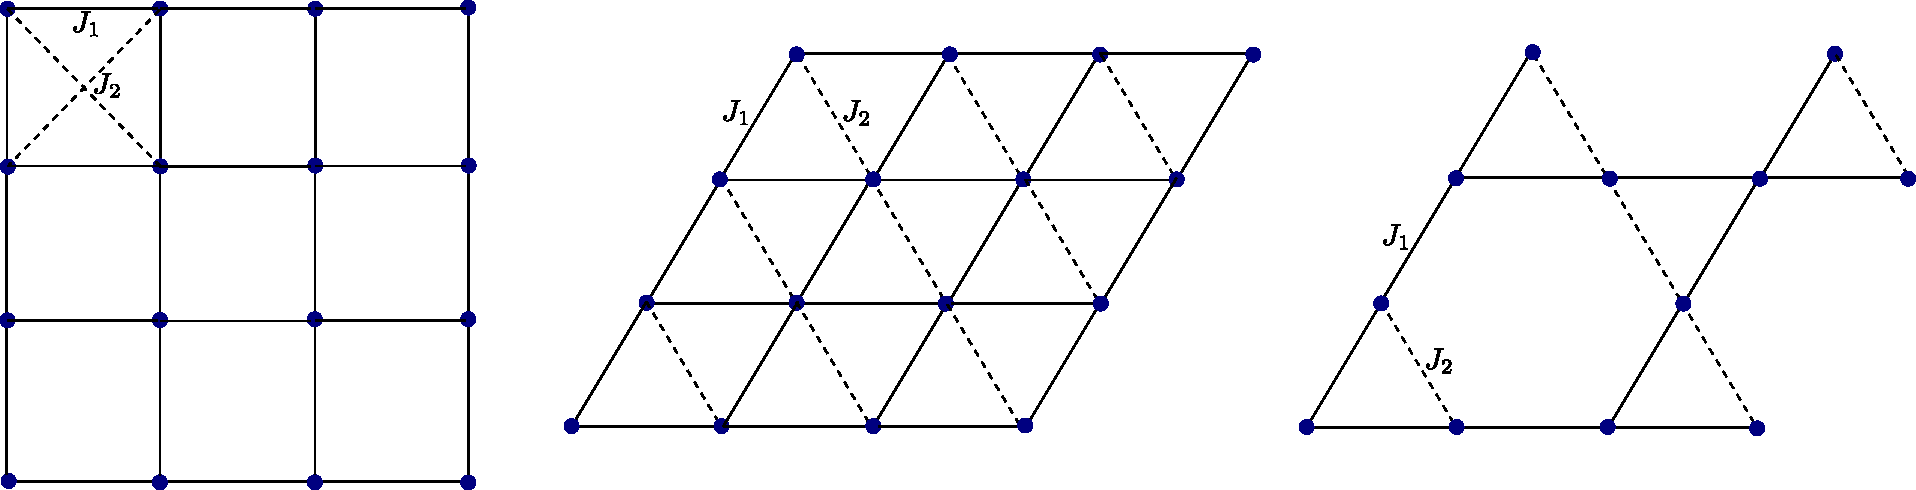
\includegraphics[width=0.95\linewidth]{figures/three_latt.pdf}};
                \node at (-19, 7.5) {Square lattice};
                \node at (0, 7.5) {Triangular lattice};
                \node at (19, 7.5) {Kagome lattice};
            \end{tikzpicture}
        \end{figure}

        \begin{textblock}{4.2}(5.5,0.22)
            \centering Ground state wavefunction
            \begin{figure}[h]
            \begin{tikzpicture}
                \node (eqn) at (0, 0) {%
                    $\displaystyle |\Psi_{GS}\rangle = \sum\limits_{i=1}^{K} \psi_i|{\mathcal S}_i\rangle
                                                     = \sum\limits_{i=1}^{K} s_i |\psi_i|\,|{\mathcal S}_i\rangle
                    $};
                \node (sgn) at (2, -4) {\small sign};
                \node (amp) at (8, -5) {\small amplitude};
                \draw[line width=0.15cm, color=black!40, -{Latex}] (2, -3.4) -- (4.6, -1);
                \draw[line width=0.15cm, color=black!40, -{Latex}] (8, -4.0) -- (5.9, -1);
            \end{tikzpicture}
            \end{figure}
        \end{textblock}

        \begin{textblock}{4.6}(0,0.22)
            \centering Heisenberg Hamiltonian
            \vspace{-1.9cm}
            \begin{figure}[h]
            \begin{tikzpicture}
                \node (eqn) at (6, 5) {\parbox{\linewidth}{\large
                    \begin{equation*}
                        \hat H = J_1 \sum_{\langle a, b \rangle}
                                     \hat{\boldsymbol{\sigma}}_a \otimes \hat{\boldsymbol{\sigma}}_b
                               + J_2 \sum_{\langle \langle a, b \rangle \rangle}
                                     \hat{\boldsymbol{\sigma}}_a \otimes \hat{\boldsymbol{\sigma}}_b
                    \end{equation*}}};
                \node[text width=15cm] (first) at (-1, -0.4) {\small
                    Sum runs over the unfrustrated sublattice (solid lines)};
                \node[text width=18cm] (second) at (20, -1) {\small
                    Sum runs over the sublattice which brings in frustrations
                    (dashed lines)};

                \draw[line width=0.15cm, color=black!40, -{Latex}] (-2.0, 1.2) -- (-0.3, 3.0);
                \draw[line width=0.15cm, color=black!40, -{Latex}] (18, 0.5) -- (11.5, 3.0);
            \end{tikzpicture}
            \end{figure}
        \end{textblock}
    \end{block}
\end{textblock}

\begin{textblock}{9.5}(5,4.7)
    \begin{block}{Varying Frustration Level}
        \centering
        $J_2/J_1 \!= \!0$ and $J_2/J_1 \!= \!\infty$ both correspond to unfrustrated regimes. \\
        Perfect generalization means overlap $=1$.

        \begin{figure}[h]
            \centering
            \input{j2_dependance}
        \end{figure}
    \end{block}

    \vspace{0.3cm}
    \begin{alertblock}{Result 1 \& 2}
        \begin{itemize}
            \item[$\bullet$] Generalization from a relatively small subset of
                the Hilbert space basis of the wavefunction sign structure is
                not granted even when the ansatz is able to express the ground
                state with high accuracy. Very well known to machine learning
                practitioners, this fact is also valid for spin systems, in both
                frustrated and ordered phases.

            \item[$\bullet$] Construction and training of a network to achieve good generalization,
                a task which is relatively simple in the ordered phase, becomes much harder in
                frustrated region.
        \end{itemize}
    \end{alertblock} 
\end{textblock}

\begin{textblock}{7.3}(0.15,10.25)
    \begin{block}{Amplitudes vs. Signs}
        \begin{textblock}{4.5}(0, 0)
        \begin{figure}[h]
            \vspace{0.5cm}
            \center
            \input{amp_vs_sign}
        \end{figure}
        \end{textblock}

        \begin{textblock}{2.9}(4.1, 0.15)
        \begin{alertblock}{Result 3}
            Predicting wavefunction amplitudes is substantially easier than
            predicting signs.
        \end{alertblock} 
        \end{textblock}
    \end{block}

\end{textblock}

\begin{textblock}{7.3}(7.5,10.25)
    \begin{block}{More Data?}
        \begin{textblock}{4.5}(0, 0)
        \begin{figure}[h]
            \center
            \input{eps_dependance}
        \end{figure}
        \end{textblock}

        \begin{textblock}{2.7}(4.3, 0.15)
        \begin{alertblock}{Result 4}
            Generalization quality depends on the size of the training dataset
            in an abrupt way exhibiting a sharp increase at some critical
            fraction $\varepsilon$.
        \end{alertblock} 
        \end{textblock}
    \end{block}
\end{textblock}

\begin{textblock}{4.6}(5.2,13.3)
    \center
    \begin{tikzpicture}
        \node[draw, line width=1.5mm, color=black!60] at (0, 0) {\url{https://arxiv.org/pdf/1907.08186.pdf}};
    \end{tikzpicture}
\end{textblock}

\end{document}

